\chapter{Analyzing Performance Through Formal Methods}
\label{cha:analyzing_rel_work}
The most common use of formal methods in relation to cache coherence is to
validate protocol correctness (i.e.~that a protocol verifies the properties set
in Section~\ref{sec:proper_cache_coherence_protocol}).  Indeed, the use of model
checking for that purpose is the source of many publications. For example,
\cite{conchon13jfla} describes a parameterized model checker by focusing on the
verification of a cache coherence protocol, by taking its description from yet
another paper using model checking to verify it (\cite{Baukus2002}) and thus
allowing a comparison between the approaches.

However, proving the correctness of a cache coherence protocol is not the
subject of this thesis. We assume the protocols to be correct, and are instead
interested by the impact the cache coherence has on the real-time properties
of the system. Thus, in chapter, we look at real-time systems using
formal methods to analyze the real-time properties of an architecture. As this
is a fairly restrictive criterion, the results include approaches meant for
single-core processors in addition to those for the more on-topic multi-cores.

\section{Single-Core Processors}
\stopallthesefloats
\subsection{METAMOC}
\begin{figure}[hbt]
\begin{center}
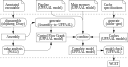
\includegraphics[width=\textwidth]{\chapterdirectory/figure/analysis/metamoc.pdf}
\end{center}
\caption{Using METAMOC to compute WCET (from
\cite{dalsgaard_et_al:OASIcs:2010:2831})}%
\label{fig:formal_analysis:metamoc}
\end{figure}

The first tool that made use of UPPAAL for the computation of WCET by modeling
hardware was Modular Execution Time Analysis using Model Checking (METAMOC),
introduced in \cite{dalsgaard_et_al:OASIcs:2010:2831}. The general idea behind
the approach is shown in Figure~\ref{fig:formal_analysis:metamoc}. The
modularity can clearly be seen in how the models for the cpu pipeline,
main memory, and cache specifications are kept separate in order to facilitate
their replacement when analyzing for a different processor. The other input is
that of the analyzed executable, directly in its binary form, albeit with some
annotations regarding loop bounds.

Given these inputs, METAMOC generates a control flow graph for the program,
which is in fact yet another UPPAAL model to combine to the ones representing
the architecture. The value analysis statically determines the address of
memory elements, and is disabled if the modeled architecture does not feature
any data cache.

The pipeline model corresponds to a collection of automata, one for each stage:
\textit{fetch}, \textit{decode}, \textit{execute}, \textit{memory}, and
\textit{writeback}. The parallel nature of pipelines translates fairly well
into a network of automata communicating through channels, making the writing
of such automata accessible for the user wanting to add their own in hopes of
modeling another architecture. The main challenges then come in determining
what can stall the pipeline on the real architecture and how long each stage
should take. Indeed, the authors of \cite{dalsgaard_et_al:OASIcs:2010:2831}
indicate that the documentation for the processor they modeled explicitly
states that it does not contain an exhaustive list of all possible stalls.

The default model for caches considers separate instructions and data caches,
matching the architecture they made their approach around. Caches are
set-associative, and implement an LRU eviction policy.

\begin{figure}[hbt!]
\begin{center}
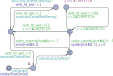
\includegraphics[width=0.8\textwidth]{\chapterdirectory/figure/analysis/half_metamoc_cache.pdf}
\end{center}
\caption{Half of Cache in METAMOC (adapted from \cite{dalsgaard_olesen_toft_2020})}%
\label{fig:formal_analysis:metamoc_caches}
\end{figure}

Figure~\ref{fig:formal_analysis:metamoc_caches} shows one half of the automaton
modeling a cache in METAMOC. The complete automaton has a second half mirroring
this one, with \textit{read} instead of write. Upon receiving a request for
a cache write, the automaton determines from its internal state whether the
request is a cache hit or if the instruction must be added to the cache. This
corresponds to \lstinline{cache_contents(instrArd)} being equal to -1 (cache
miss) or not (cache hit). In the case of a cache hit, a delay corresponding to
the time spent writing in the cache is introduced (controlled by
the \lstinline{CACHEFETCH} clock). \lstinline{write_hit_wait} corresponds to
the number of main memory accesses to be performed. Such accesses can still
occur even after a cache hit, if a write-through policy is in place. In the
case of a cache miss, a number of accesses to the main memory are performed.
This number can be higher than one if a cache line had to be evicted and the
cache follows a write-back policy. Once all accesses are performed, the cache
synchronizes on \textbf{instructionCacheWrite} to indicate that the request
was completed.

\begin{figure}[hbt!]
\begin{center}
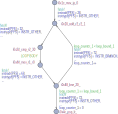
\includegraphics[width=0.8\textwidth]{\chapterdirectory/figure/analysis/metamoc_prog.pdf}
\end{center}
\caption{Fragment of Program Automaton in METAMOC (from \cite{dalsgaard_olesen_toft_2020})
}
\label{fig:formal_analysis:metamoc_program}
\end{figure}

Figure~\ref{fig:formal_analysis:metamoc_program} shows an example fragment of
an automaton corresponding to a program after processing by METAMOC. The
fragment in question corresponds to a loop, and shows how METAMOC supports
branching and iterating. The \textit{loop\_counter\_1} and
\textit{loop\_bound\_1} variables ensures that its execution terminates. The
bounds of such loops have to be annotated in the program's source code.

Their solution to limit search-space explosion is to put a caveat stating that
the architectures are assumed to be time-anomaly free, which lets them consider
only the locally worst time for some operations, instead of having to explore
all possible timings in case a better local time leads to a globally worse one.

\stopallthesefloats

\stopallthesefloats
\subsection{WUPPAAL}
\begin{figure}[hbt]
\begin{center}
\centering
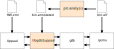
\includegraphics[width=0.7\textwidth]{\chapterdirectory/figure/analysis/wuppaal.pdf}
\end{center}
\caption{Overview of WUPPAAL's components (taken from \cite{wuppaal})}%
\label{fig:formal_analysis:wuppaal}
\end{figure}

\cite{wuppaal} describes WUPPAAL, another approach to using UPPAAL in order to
compute the WCET of a program running on a single-core processor. The main
novelty of \cite{wuppaal} is that it combines simulated execution with the
model checking. Indeed, as can be seen in
Figure~\ref{fig:formal_analysis:wuppaal}, it allows UPPAAL to interact with
\textit{qemu} (an architecture simulation tool) through \textit{gdb} (a
debugging tool) and \textit{libgdbuppaal} (a library of their own making). The
\textit{pre-analysis} step shown in the figure corresponds to the annotation of
a binary program with information in order to help the extraction its
\textit{Control Flow Graph}. This approach aims at improving the memory usage
of model checking, as well as making the approach fit other architectures very
easily (by just changing qemu parameters).

These annotations allow the generation of an over-approximation of all valid
program runs from the CFG. This has some surprising results, such as
deterministic programs having multiple separate runs because the
over-approximation does not consider actual values for any computation
involving input parameters. Instead, all outcomes are considered, even if some
sequences of outcomes cannot follow one another (e.g.~the exact same test
failing once, then succeeding). For such runs to be finite, loops cannot be
controlled by input parameters (i.e.~all loops have a known amount of
iterations).

\begin{figure}[hbt]
\begin{center}
\centering
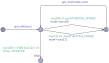
\includegraphics[width=0.7\textwidth]{\chapterdirectory/figure/analysis/wuppaal_automaton.pdf}
\end{center}
\caption{Automaton interacting with \textit{libgdb2uppaal} (taken from
\cite{wuppaal})}%
\label{fig:formal_analysis:wuppaal_automaton}
\end{figure}

UPPAAL is used to perform queries among all possible execution paths. However,
in WUPPAAL, the automaton corresponding to the program is not a purely UPPAAL
one. Figure~\ref{fig:formal_analysis:wuppaal_automaton} shows the automaton in
question.  It does not store full program states, and instead only keeps an
identifier and the annotations for current instruction. The function calls seen
on the automaton actually trigger another component from
Figure~\ref{fig:formal_analysis:wuppaal}: \textit{libgdbuppaal}. This component
is where program states are stored. \textit{libgdbuppaal} uses \textit{qemu} to
compute the program state resulting from the application of the instruction, as
well as all possible next execution nodes. The program state inserted back in
UPPAAL indicates whether the instruction was found in the cache and how long its
execution stage lasts.

UPPAAL is then involved in the computation of the WCET for these annotated
traces. Indeed, it models the pipelines, with one automaton per stage, as well
as a main memory automaton and an instruction cache one (see
Figure~\ref{fig:formal_analysis:wuppaal_cache}), to model their access times.
Since the information about whether the instruction cache contains the
instruction or not is already in the annotated execution trace, these last two
automata are kept very simple.

\begin{figure}[hbt]
\begin{center}
\centering
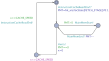
\includegraphics[width=0.7\textwidth]{\chapterdirectory/figure/analysis/wuppaal_cache.pdf}
\end{center}
\caption{WUPPAAL Instruction Cache Automaton (taken from
\cite{wuppaal})}%
\label{fig:formal_analysis:wuppaal_cache}
\end{figure}

Figure~\ref{fig:formal_analysis:wuppaal_cache} shows the automaton
corresponding to an instruction cache in WUPPAAL. The initial state is the top
one. Upon receiving a request for reading on \textbf{InstructionCacheReadStart}
(considering the rest of the variables, writing likely uses the same channel),
the automaton checks if the information is already in the cache. If not it
performs as many synchronizations with the main memory automaton as is needed
(indicated by \textit{PMT}), then waits a time corresponding to that of a
cache access before using \textbf{InstructionCacheReadEnd} to signal the
completion of the request.

\stopallthesefloats


\section{Multi-Core Processors}
\stopallthesefloats{}
\subsection{Modeling Shared Buses}
\begin{figure}[hbt!]
\begin{center}
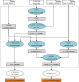
\includegraphics[width=0.7\textwidth]{\chapterdirectory/figure/analysis/mingsong.pdf}
\end{center}
\caption{Overall strategy for \cite{5702243} (taken from the paper)}%
\label{fig:formal_analysis:mingsong}
\end{figure}

The approach proposed by \cite{5702243} combines abstract interpretation and
model checking to compute WCET in multicore, with a special focus on the
interconnect. The abstract interpretation is found in the analysis of the
caches, which is done in a fashion similar to those presented in
Section~\ref{sec:rel_work:handling_it:accepting_it}, including in its remarks
of a previous approach being unsafe and in its omission of data caches (and
thus, of cache coherence). The overall strategy for this approach is shown in
Figure~\ref{fig:formal_analysis:mingsong}.

\begin{figure}[hbt!]
\begin{center}
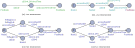
\includegraphics[width=\textwidth]{\chapterdirectory/figure/analysis/mingsong_program_block.pdf}
\end{center}
\caption{Program Model Building Blocks (taken from \cite{5702243})}%
\label{fig:formal_analysis:mingsong_prog_blocks}
\end{figure}

\begin{figure}[hbt!]
\begin{center}
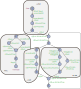
\includegraphics[width=\textwidth]{\chapterdirectory/figure/analysis/mingsong_program.pdf}
\end{center}
\caption{Program Example (adapted from \cite{5702243})}%
\label{fig:formal_analysis:mingsong_program}
\end{figure}

The resulting model considers program instructions only as their categorization
(\textit{Always Hits}, \textit{Always Misses}, \textit{First time Misses},
\textit{Not Categorized}). The paper proposes an automaton for each category
(see Figure~\ref{fig:formal_analysis:mingsong_prog_blocks}),
indicating how an instruction of this category will use the
interconnect. Models for program are thus constructed by replacing each
instruction in the control flow graph by the automaton corresponding to its
synchronization with the interconnect
(\textit{TA Construction} in Figure~\ref{fig:formal_analysis:mingsong}). An
example of resulting automaton can be seen in
Figure~\ref{fig:formal_analysis:mingsong_program}.

To showcase how modular the approach is in its modeling of the interconnect,
\cite{5702243} provides both a model for a TDMA bus and for a FCFS
(\textit{First Come, First Served}, which means requests are completed in the
order of their arrival) bus.

Figure~\ref{fig:formal_analysis:mingsong} mentions an ILP model being computed
as well, however, the paper does not make any mention of it.

\stopallthesefloats{}

\stopallthesefloats
\subsection{Multi-Core Analysis using only UPPAAL}
The authors \cite{conf/wcet/GustavssonELP10} present an approach using UPPAAL
to perform computation of the worst-case execution time for software running
on multi-core processors. While it does not feature cache coherence, it does
support hierarchical (and shared) caches, as well as some sort of instruction
pipelining.

\begin{figure}[hbt!]
\begin{center}
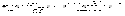
\includegraphics[width=\textwidth]{\chapterdirectory/figure/analysis/gustavsson_prog.pdf}
\end{center}
\caption{Program Automaton (taken from \cite{conf/wcet/GustavssonELP10})}%
\label{fig:formal_analysis:gustavsson_program}
\end{figure}

In \cite{conf/wcet/GustavssonELP10}, programs are represented by their own
automata (See Figure~\ref{fig:formal_analysis:gustavsson_program}), sending
instructions through shared variables by synchronizing with a core on
a dedicated channel. This approach allows programs to feature branching and
non-memory-related instructions, by simply adding numerical variables and
making the automaton more than a simple sequence of states. In
Figure~\ref{fig:formal_analysis:gustavsson_program}, the framed part corresponds
to where the program's instruction graph should be. The \textit{id} variable
targets a particular core on which to execute the instruction, and
\textit{set\_access\_info} populates the global variables characterizing the
instruction: \textit{instr\_address} for the address of the instruction in the
modeled memory, \textit{data\_address} for the address of any data being
accessed, \textit{data\_access} to indicate if this instruction accesses data,
and \textit{write\_data} to differentiate between a read and a write access.
The \textit{Terminating Synchronization} part is here to ensure the task is not
considered completed until it has indeed completed all accesses for its final
instruction (and not just sent the instruction).

Cores are modeled as automata that go through the pipeline required for an
instruction to be completed, which includes accessing the instruction cache as
well as, potentially, the data cache. Interestingly enough, this model does not
use one automaton per stage of the pipeline. Instead the whole core logic is
modeled in a single automaton.


\begin{figure}[hbt!]
\begin{center}
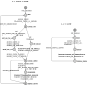
\includegraphics[width=\textwidth]{\chapterdirectory/figure/analysis/gustavsson_caches.pdf}
\end{center}
\caption{Cache Automata (taken from \cite{conf/wcet/GustavssonELP10})}%
\label{fig:formal_analysis:gustavsson_caches}
\end{figure}

Each L1 instruction cache has its own automaton, managing the possibility for
instructions to have already been cached or sending a request for that
instruction to the L2 cache. The L1 data caches are similar (see
Figure~\ref{fig:formal_analysis:gustavsson_caches}), with the added possibility
of writing data to a memory element, which invalidates it from every other L1
data cache.

The automaton for the L2 cache is very straightforward, a simple loop going
over each request, determining whether the data is supposed to be in the L2
cache or not, and delaying the reply accordingly.

\iffalse
An extra automaton is also provided, which acts as a mutex for use in modeling
the programs.
\fi

Unsurprisingly, the hampering factor is scalability when the number of modeled
cores is increased. There appear to have very little in the way of synchronicity
between the cores (such as using a round-robin for L2 cache accesses), which
is likely to be aggravating the issue.
\stopallthesefloats


\section{Conclusion}
This chapter has shown how UPPAAL's model checking capabilities can be exploited
to analyze the interference caused by cache coherence on the model from
Chapter~\ref{cha:modeling_cache_coherence}.

This analysis starts by a computation of the WCET for each program. Useful in
itself, this analysis is extended by that of the WCET for these programs with
the architecture in different configurations in order to extract more
information about how much of the execution time is caused by interference.

In order to more precisely understand what determine the WCET and to provide
the user with information about elements of the program that can directly be
manipulated, the analysis proceeds by an categorization of the accuracy of each
instruction. This indicates which instructions are unaffected by the
interference, which instructions are always time-consuming, and which
instructions take a varying amount of time depending on the execution. By
looking at the accuracy of all accesses made on each memory element, patterns
for these instructions of varying execution time can sometimes be found, which
results in a more predictable system.

The determining factor for the accuracy of instructions is then properly
defined. This corresponds to a categorization of all external queries depending
on their effects on the permissions held by a cache, and whether a loss of
permission led to an instruction taking additional time. Thus, three categories
of interference are defined: minor (no change of permission, but loss of time
due to query processing), demoting (loss of writing permission), and expelling
(loss of all permissions).

Finally, analyses are performed in order to determine how each instruction
interfere with the other instructions. This results in a graph showing, for
each instruction, which instruction can generate interference that will
directly impact it, the category of this interference, and whether this
interference occurs on all possible executions or not.

This provides the user with a clear understanding of the causes and effects of
cache coherence interference on the programs' instructions, opening the way to
finding means of mitigation for this interference.

